\chapter{Simulation tests} %Preliminary Results
\section{Bunch parameters}
The initial phase of this project involves simulating beam dumping of a proposed electron beam for the EuPRAXIA project. This is a European Union Horizon 2020 research project with the aim of developing a conceptual design report for a high-quality compact 5 GeV electron plasma wakefield accelerator for application in research and medicine \cite{Eupraxia}. Currently the studies are concerned with achieving high-quality 1 GeV electron beams. As the simulations and experiments yield successful results at this energy, higher energies will be expolored until the 5 GeV goal is reached. Current target values for the electron bunch parameters are given in table \ref{eupraxia_parameters}, where case 1 and 2 represents laser-driven and beam-driven driven accelerators respectively \cite{Eupraxia}.  In addition, parameters are shown for the simulated 1 GeV electron beam that we aim to dump. These differ in two key aspects from the other EuPRAXIA cases. Firstly, the energy spread and emittance of the bunch have been lowered. This lowers the computational cost of running these simulations, by effectively decreasing the relative motion of the particles in the bunch, while still maintaining a realistic beam quality \cite{Walker2017}. Secondly, the size of the bi-Gaussian bunch has been increased significantly because of the fact that the current parameters would lead to peak bunch-densities in excess of $10^{20} \text{cm}^{-3}$, making neither linear nor quasilinear ($n_p=n_b$) regimes accessible with conventional plasma sources. Plasma densities $\sim 10^{20} \text{cm}^{-3}$ are achievable using supersonic gas jets \cite{Schmid2012} -- where a a high-density gas jet is ionised into a plasma using a laser -- however the novelty and impracticality of this technique lead us to instead lower the bunch density. Expansion of the bunch in the radial direction could be achieved by simply letting the bunch propagate freely in a vacuum, at which point the bunch would expand due to its space-charge force, while longitudinal stretching is achievable using conventional so-called magnetic chicanes \cite{Maier2012}. We choose here to expand the dimensions of the bunch to $\sigma_{\xi}=\sigma_r=5~\mu\text{m}$. This is chosen in part to give a more workable bunch density of $n_b=10^{17} \text{cm}^{-3}$, as well as to allow for comparisons with existing free-electron laser and plasma wakefield experiments, which tend to have bunch dimensions in the single to tens of micrometer range. \vspace{-10pt}\\
\begin{table}[!ht]
\centering
\includegraphics[width=0.85\textwidth]{table_eupraxia.pdf}
\caption{\small{Parameters for the accelerated electron bunch in the EuPRAXIA project for laser-driven  (case 1) and beam-driven (case 2) plasma wakefield accelerators. Parameters for the simulated beam used in our hybrid scheme study are also shown.}}
\label{eupraxia_parameters}
\end{table}

\section{Linear and quasilinear regimes}
\begin{figure}
\centering
%\includegraphics[width=0.49\textwidth]{Energies30pc_lowres.pdf}
\includegraphics[width=0.85\textwidth]{Energy30pc_per_particle_lowres2.pdf}
\caption{\small{Fractional remaining energy per particle as a function of propagation distance through uniform plasmas in the linear ($n_p=n_b$) and quasilinear ($n_p=10n_b$) regimes. The simulated electron bunch parameters are given in table \ref{eupraxia_parameters}.}}
\label{energyloss}
\end{figure}
In this section we present results for simulations in the linear regime, where the plasma density $n_p=10n_b$, and the quasilinear regime, where $n_p=n_b$, for the bunch parameters given  in table \ref{eupraxia_parameters}. The remaining fraction of the initial bunch energy, per particle, for this bunches is plotted in figure \ref{energyloss} as a function of the propagation distance through these two plasmas. We note that, as found by Wu et al. \cite{Wu2010}, the energy loss in both regimes decreases linearly until the energy saturates at around 30-40\%. We further note that saturation is reached faster in the linear regime than in the quasilinear regime, which is simply due to the fact that the magnitude of the decelerating field given by equation (\ref{longitudinalforce}) scales linearly with the plasma density. It is instructive to look at both these regimes in further detail.\\
\indent Figure \ref{linearplots} shows the longitudinal wakefield, the longitudinal energy distribution and spatial distribution of the linear bunch at two positions. Specifically, at (a) 20cm, when the energy is starting to level off, and (b) 48cm, when the energy is fully saturated. At both positions there is a clear energy chirp at the head of the bunch which experiences a near-zero electric field. In figure (a) we also see clear signs of re-acceleration, where particles in the bunch has been decelerated, fallen behind, and gotten caught in two regions: where the sign of the electric field changes and the minimum of the electric field. In figure (b) the bunch has split into four distinct parts and we note a low-energy tail around $\xi=-20 \mu\text{m}$. This could potentially be removed using absorbing material as we described in figure \ref{hybrid_outline}. The large central re-acceleration peak however is not suitable for the hybrid scheme we have in mind; since we seek a single energy peak to dump with a laser. A solution to this issue is to increase the wavelength of the longitudinal wakefield by lowering the plasma density, which takes us into the quasilinear regime. \\
\indent The linear simulations where conducted with a grid size of $1 \mu\text{m}\times 1\mu\text{m}$, each grid point populated with 6 macroparticles and the simulation ran on 24 cores for 72 hours. This proved sufficient to resolve the bunch and the plasma wavelength with enough grid points to ensure that all small-scale phenomena were accounted for. When the same resolution was used for the quasilinear simulations we encountered large transverse inabilities. Figure \ref{cherenkov} shows the emergence of the instabilities and the resulting disintegration of the bunch. This beam dispersion appeared at first to be a promising approach for rapid beam deceleration. Indeed, several beam instabilities are known to occur in beam-driven plasma wakefield acceleration. The \textit{hosing instability} \cite{Huang2007} exhibits similar formation as in figure \ref{cherenkov} and therefore appeared a good candidate. However, in discuss with colleagues it was found that this is likely to be a numerical artefact in the PIC code known as the \textit{numerical Cherenkov instability}. This is in fact a prevalent numerical issue in all relativistic PIC codes \cite{Godfrey2018}. It arises in the PIC loop, described in figure \ref{PIC_loop}, as a result of the different treatment of particles and fields  \cite{Blinne}. This introduces deviations from the correct velocities of the particles in the beam, which  leads to unphysical emission of Cherenkov radiation \cite{Godfrey2018}. It appears that these emissions introduce microscopic instabilities which are amplified by the collective motion of the electrons. Although several grid and algorithm modifications exist in EPOCH to reduce these effects, there is no secure way to avoid them other than to increase the grid and macroparticle resolution. A grid size of $0.1 \mu\text{m}\times 0.1\mu\text{m}$, with each grid point populated with 10 macroparticles proved successful in mitigating these effects. 
\begin{figure}
\centering
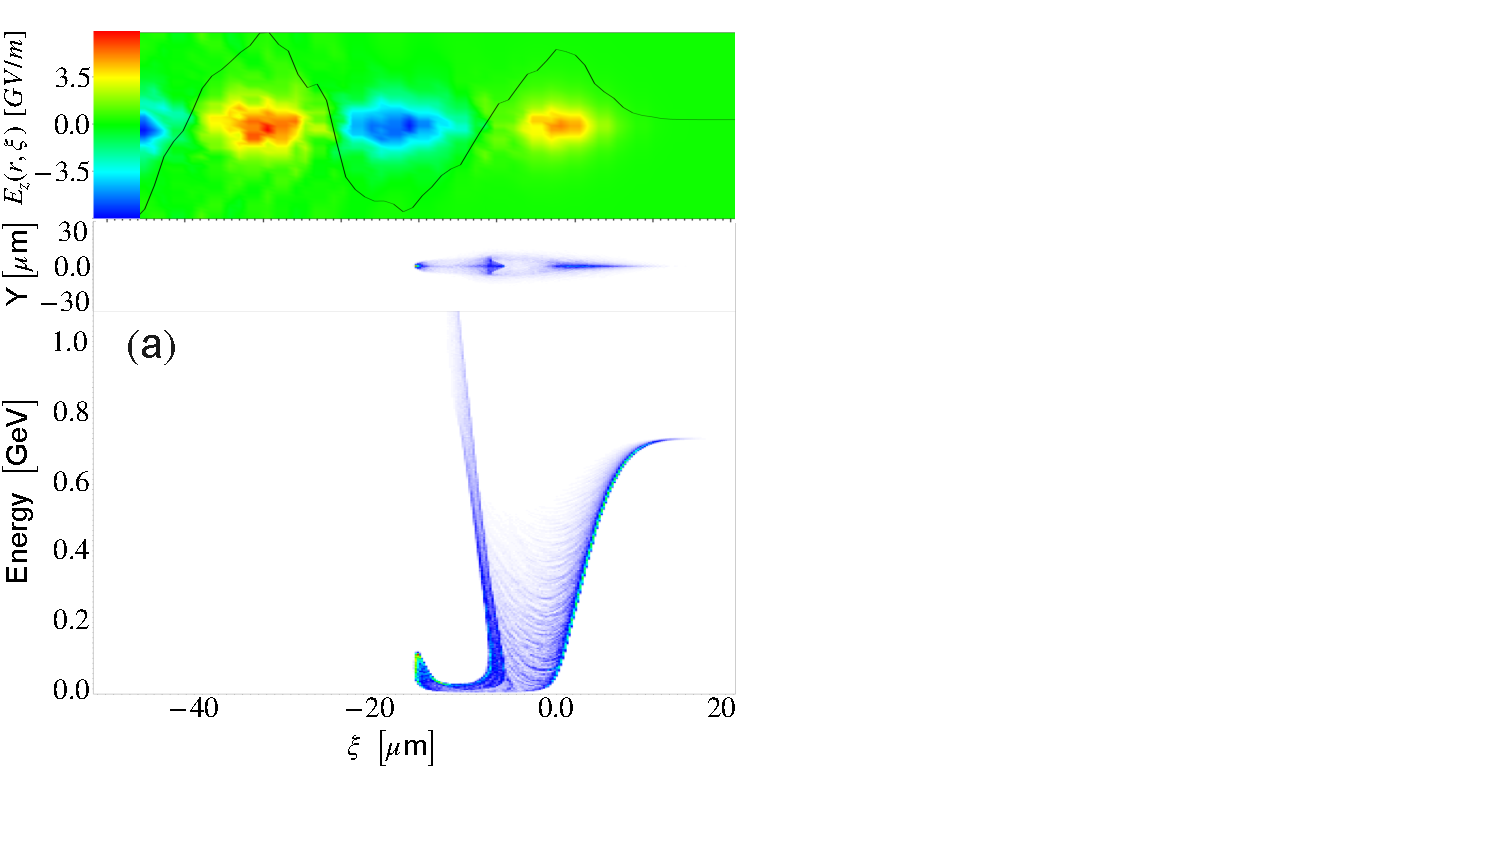
\includegraphics[width=0.47\textwidth]{linear.pdf}\hspace{24pt}
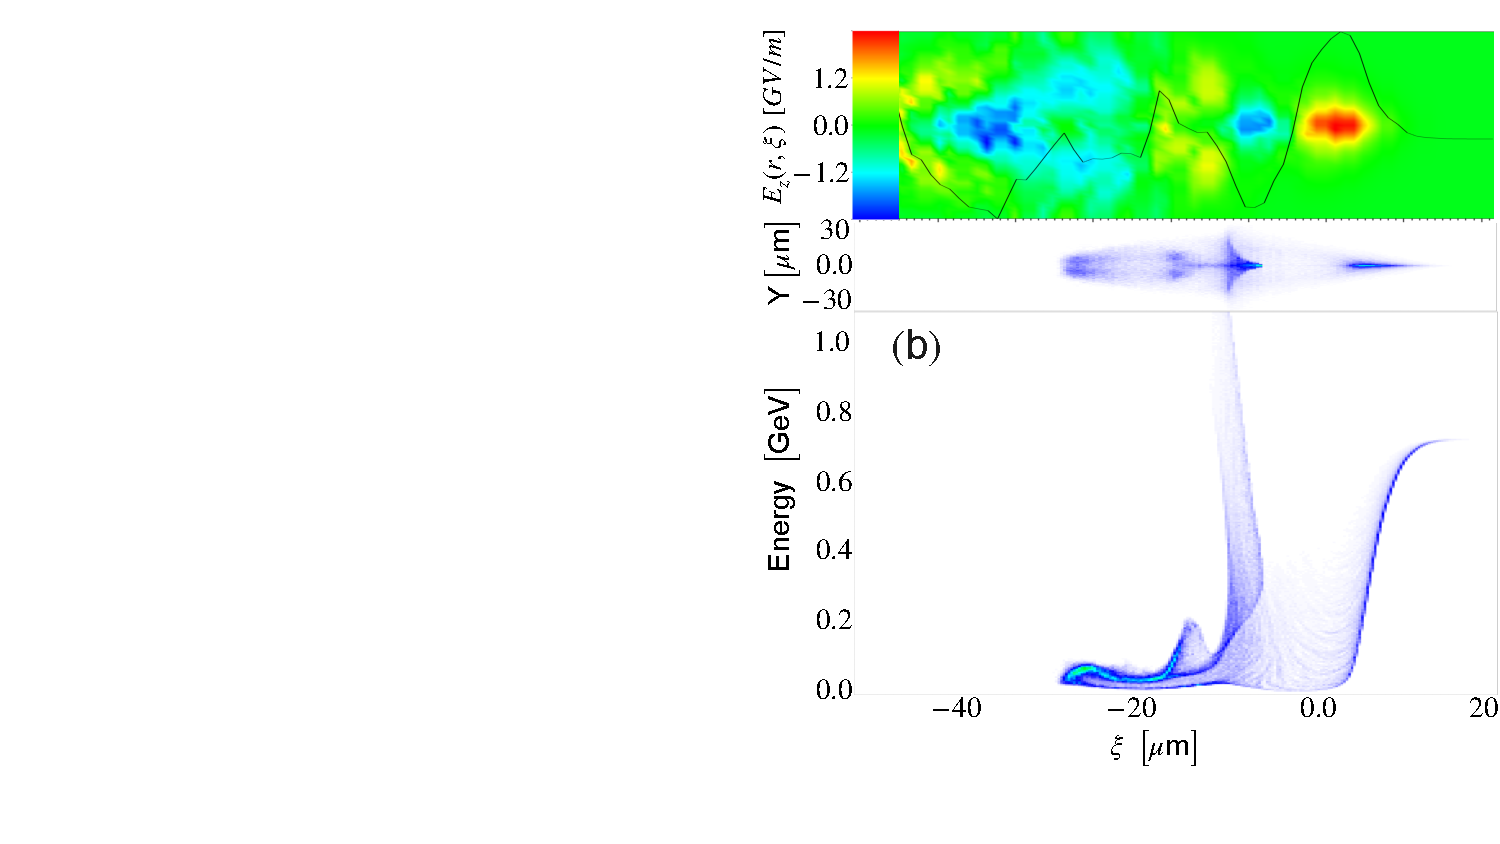
\includegraphics[width=0.47\textwidth]{linear2.pdf}
\caption{\small{Plots of (top) the co-moving longitudinal wakefield (middle) spatial distribution of the electron bunch and (bottom) longitudinal energy distribution at (a) 20 cm and (b) 48 cm in the linear regime. The bunch is moving to the right and the the color scale of the spatial and energetic distributions is the same as in figure \ref{cherenkov}.}\vspace{-5pt}}
\label{linearplots}
\end{figure}
\vspace{-4pt}\\
\begin{figure}[!ht]
\centering
\includegraphics[width=\textwidth]{cherenkov_color}
\caption{\small{Plots of the onset and result of the numerical Cherenkov instability on the spatial distribution of the electron bunch in the low-resolution quasilinear regime.}}
\label{cherenkov}
\end{figure}
\clearpage
\noindent The simulation needed to run on 24 cores for 14 days before completion. The resulting energy loss is given in figure \ref{energyloss}, with the corresponding fields and distributions given in figure \ref{quasiplots}. We note that in contrast to the linear regime, saturation now occurs through the growth of a long low-energy tail, which eventually divides the bunch into the two distinct parts. The trailing bunch in (b) peaks at 400 MeV, which is too high for removal with low-energy absorbing material or magnetic deflection, however the slow growth of the tail over 18 cm means that we can find a position around 30-40 cm where the majority of trailing particles are still non-relativistic. If we simply remove the data of these particles we find that we are left with an energy chirp, $\xi>0$, with an average energy of $300$ MeV per particle. Proper simulations would of course be necessary to verify this, but for the present the quasilinear regime appears to provide a bunch well suited for the active beam dumping phase. 

\begin{figure}
\centering
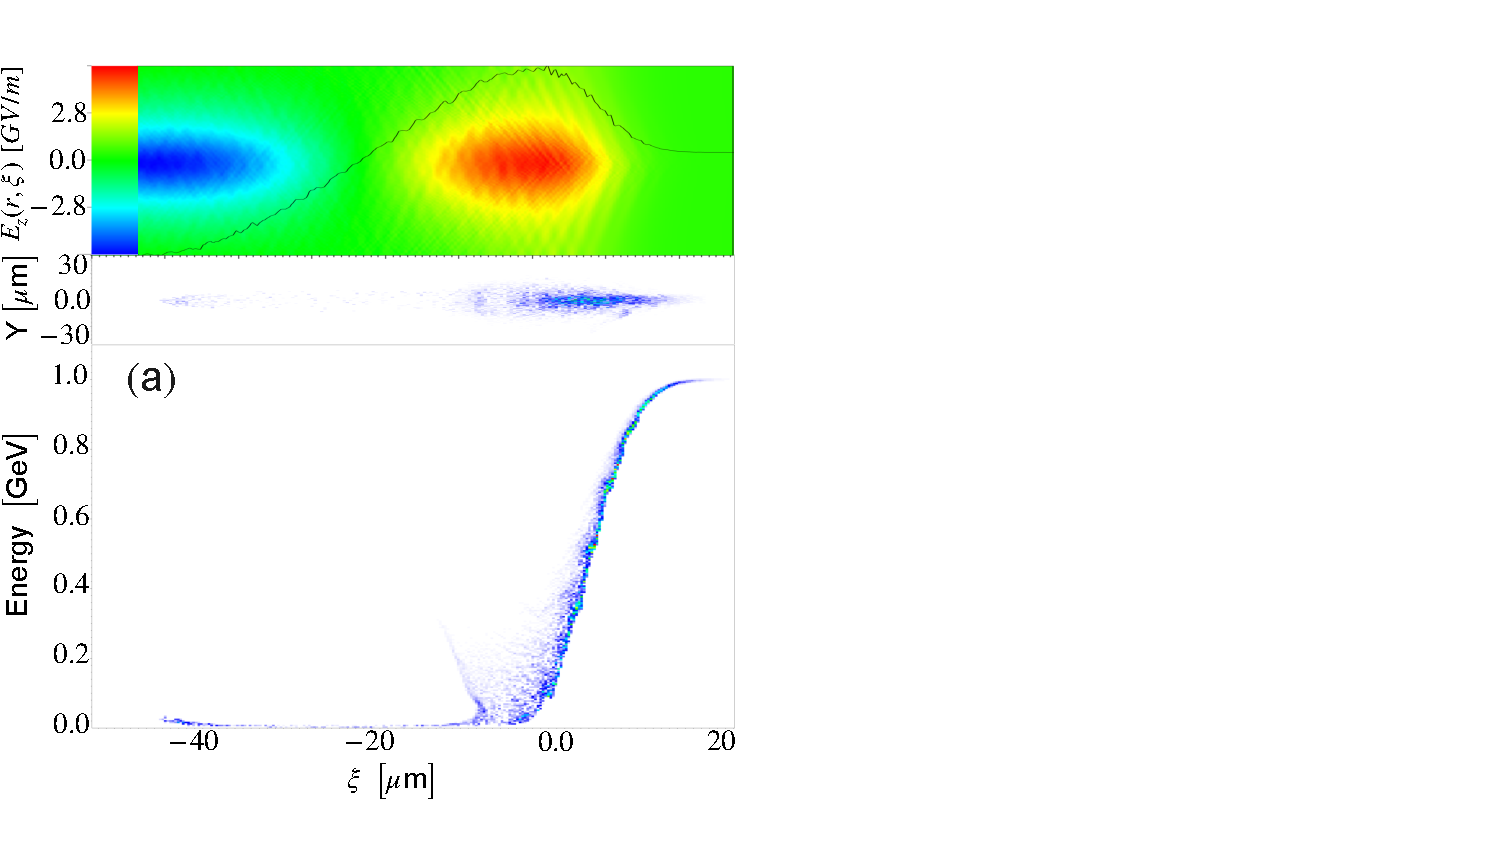
\includegraphics[width=0.47\textwidth]{quasiplots3.pdf}\hspace{24pt}
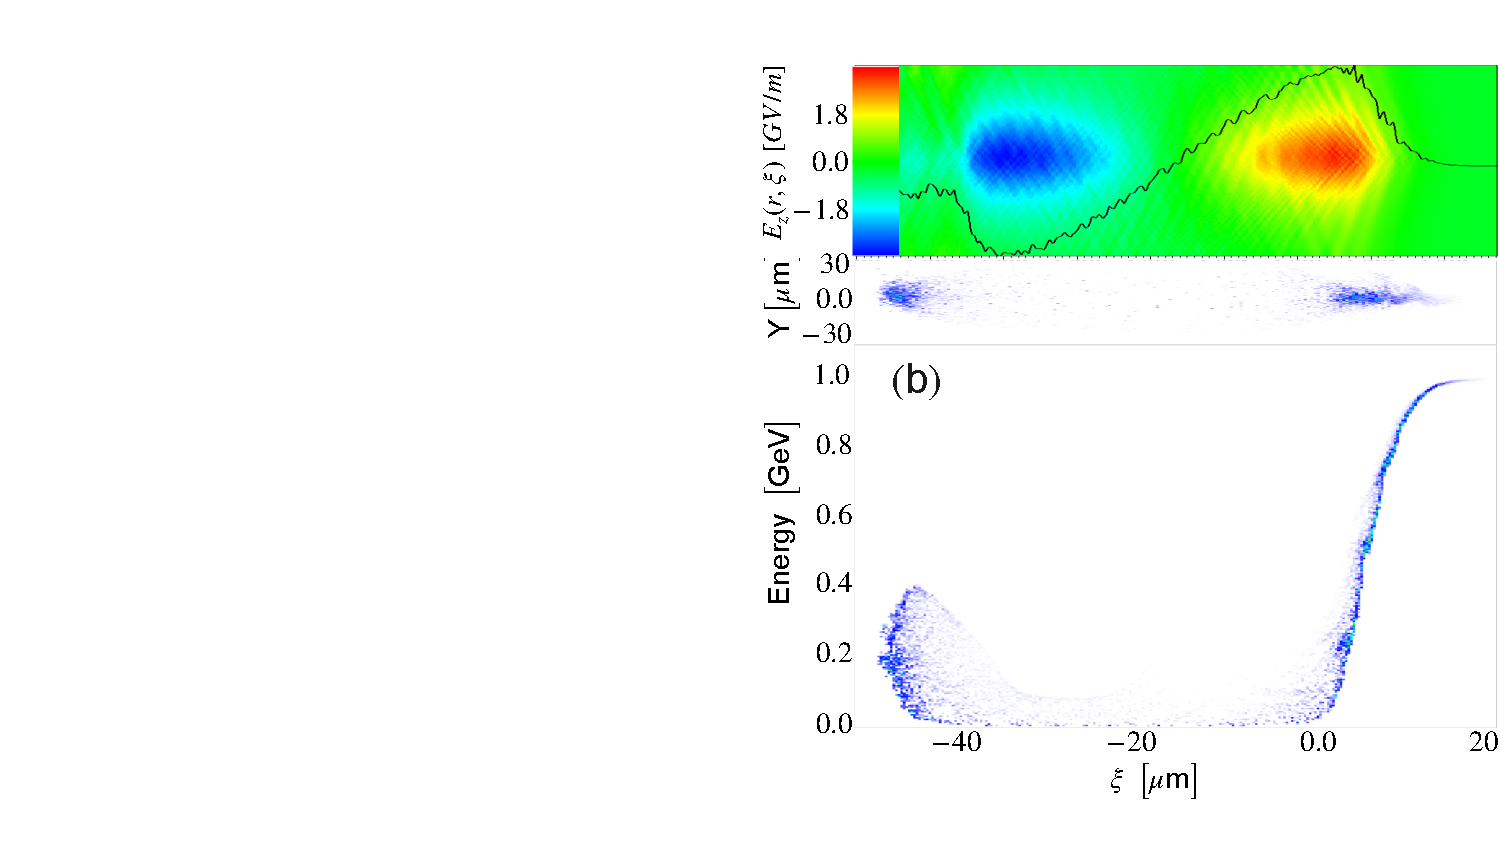
\includegraphics[width=0.47\textwidth]{quasiplots2.pdf}
\caption{\small{Plots of (top) the co-moving longitudinal wakefield (middle) spatial distribution of the electron bunch and (bottom) longitudinal energy distribution at (a) 30 cm and (b) 48 cm in the quasilinear regime. The color scale of the spatial and energetic distributions is the same as in figure \ref{cherenkov}. }}
\label{quasiplots}
\end{figure}
